\documentclass{beamer}

\mode<presentation>
{
  \usetheme[secheader]{Madrid}
  \setbeamercovered{transparent}
}

\usepackage[utf8]{inputenc}
\usepackage[spanish]{babel}
\usepackage{graphicx}
\usepackage{url}
\usepackage{times}
\usepackage[T1]{fontenc}
% \usepackage{xmpincl}
% \includexmp{metadata}
\usepackage{hyperref}
\hypersetup{pdfkeywords=open free design source hardware colombia Software Libre abierto Campus Party 2009 AltaImpedancia alta impedancia electrónica}

\title[Open Source Hardware]{Extendiendo el modelo del software libre al hardware}
\subtitle{Open Source Hardware}

\author[]{Jorge~Ernesto~Guevara~Cuenca \and Fredy~J.~Pulido~López}

\institute[\url{http://www.altaimpedancia.org}]
{ \inst{1}
  Colibri - Comunidad de Usuarios de Software Libre en Colombia\\
  \url{http://www.slcolombia.org}
  \and
  \inst{2}
  AltaImpedancia\\
  \url{http://www.altaimpedancia.org}
}

\date[Campus Party 2009]
{Campus Party 2009\\Innovación  -  Software Libre}

\subject{Open Source Hardware y Sofware Libre}

\pgfdeclareimage[height=1cm]{logo}{img/altaimpedancia}%university-logo-filename
\logo{\pgfuseimage{logo}}

\AtBeginSubsection[]
{ \begin{frame}<beamer>{Agenda}
    \tableofcontents[currentsection,currentsubsection]
  \end{frame}}

\beamerdefaultoverlayspecification{<+->}

\begin{document}

\begin{frame}
  \begin{figure}
    
\includegraphics[scale=2]{img/altaimpedancia-lanzamiento}
  \end{figure}
\end{frame}

\begin{frame}
  \titlepage
\end{frame}

\begin{frame}
  \frametitle{Agenda}
  \tableofcontents
  % You might wish to add the option [pausesections]
\end{frame}

% \begin{frame}
%   \frametitle{Objetivos}
%   Principal:
%   \begin{itemize}
%   \item Mostrar que el Open Source Hardware es una realidad.
%   \end{itemize}
%   Específicos:
%   \begin{itemize}
%   \item Presentar una descripción general de como se hace el hardware.
%   \item Definir y contextualizar el término Open Source Hardware y otros necesarios para entenderlo.
%   \item Mostrar algunos proyectos de Open Source Hardware.
%   \end{itemize}
% \end{frame}

\section<presentation>*{Extendiendo el modelo del software libre al hardware}

\begin{frame}{Objetivos}
  \begin{block}{Principal}
    Mostrar que el Open Source Hardware es una realidad.
  \end{block}
  \begin{block}{Especificos}
    \begin{itemize}
    \item Presentar una descripción general de como se hace el hardware.
    \item Definir y contextualizar el término Open Source Hardware y otros necesarios para entenderlo.
    \item Mostrar algunos proyectos de Open Source Hardware.
    \end{itemize}
  \end{block}
\end{frame}

% \begin{frame}
%   \frametitle{Glosario}
%   \begin{itemize}
%   \item HDL acrónimo de Hardware Description Language (Lenguaje de descripción de hardware).
%   \item PCB acrónimo de Printed Circuit Board (Tarjeta de circuito impreso).
%   \item VLSI acrónimo de Very Large Scale Integration.
%   \item FPGA acrónimo de Field Programable Gate Array.
%   \item Netlist, lista de conexiones.
%   \item footprint
%   \end{itemize}
% \end{frame}

\section{Como se hace el hardware}

\subsection{Lo que se necesita}

\begin{frame}{Herramientas EDA}{¿Qué es CAD?}
  \begin{itemize}
  \item CAD es el acrónimo de Computer Aided Design (Diseño asistido por computador).
  \item En principio se refiere a aplicaciones para hacer dibujos.
  \item Se usa en general para cualquier campo del conocimiento en el que se pueda diseñar por medio de un computador.
  \item ECAD es el acrónimo de Electronic Computer Aided Design (Diseño electrónico asistido por computador).
  \end{itemize}
\end{frame}

\begin{frame}{Herramientas EDA}{¿Qué es EDA?}
  \begin{itemize}
  \item EDA es el acrónimo de Electronic Design Automation (Automatización de diseño electrónico).
  \item Se refiere a todas las herramientas involucradas en el desarrollo de hardware.
  \item Es todo el software ECAD y hardware requeridos para el desarrollo de hardware.
  \item Hardware requerido
    \begin{itemize}
    \item HDK (Hardware Development Kits)
    \item HPP (Hardware Prototyping Plataforms).
    \end{itemize}
  \end{itemize}
\end{frame}

\begin{frame}{Herramientas EDA}
  \begin{itemize}
  \item Lenguajes de descripción de circuitos.
    \begin{itemize}
    \item netlist, ejemplo spice.
    \item HDL, ejemplo verilog.
    \end{itemize}
    \vspace{9pt}
  \item Captura esquemática y modelado gráfico.
    \begin{itemize}
    \item Diagramas de flujo.
    \item ASM.
    \item etc\dots{}
    \end{itemize}

    \vspace{9pt}
  \item Simuladores y visualizadores.
    \vspace{9pt}
  \item Fabricación de tarjetas de cirtuitos impresos (PCB).
  \item Fabricación de circuitos integrados (VLSI).
  \item Programación de dispositivos lógicos (FPGA, PAL, PLD).
  \end{itemize}
\end{frame}

\subsection{Como se hace}

\begin{frame}
  \begin{figure}
    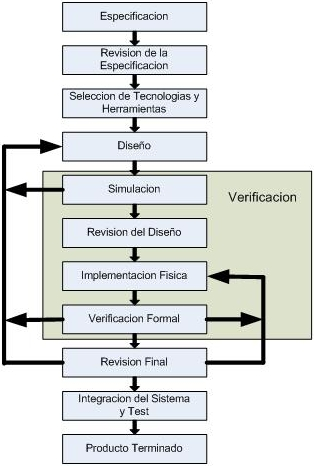
\includegraphics[scale=0.6]{img/metodologia}
    \caption{Metodología universal de diseño \cite{Guillermo}.}
    \label{fig:metodologia}
  \end{figure}
\end{frame}

\subsection{Lo que se obtiene}

\begin{frame}{Producto terminado}
  \begin{figure}
    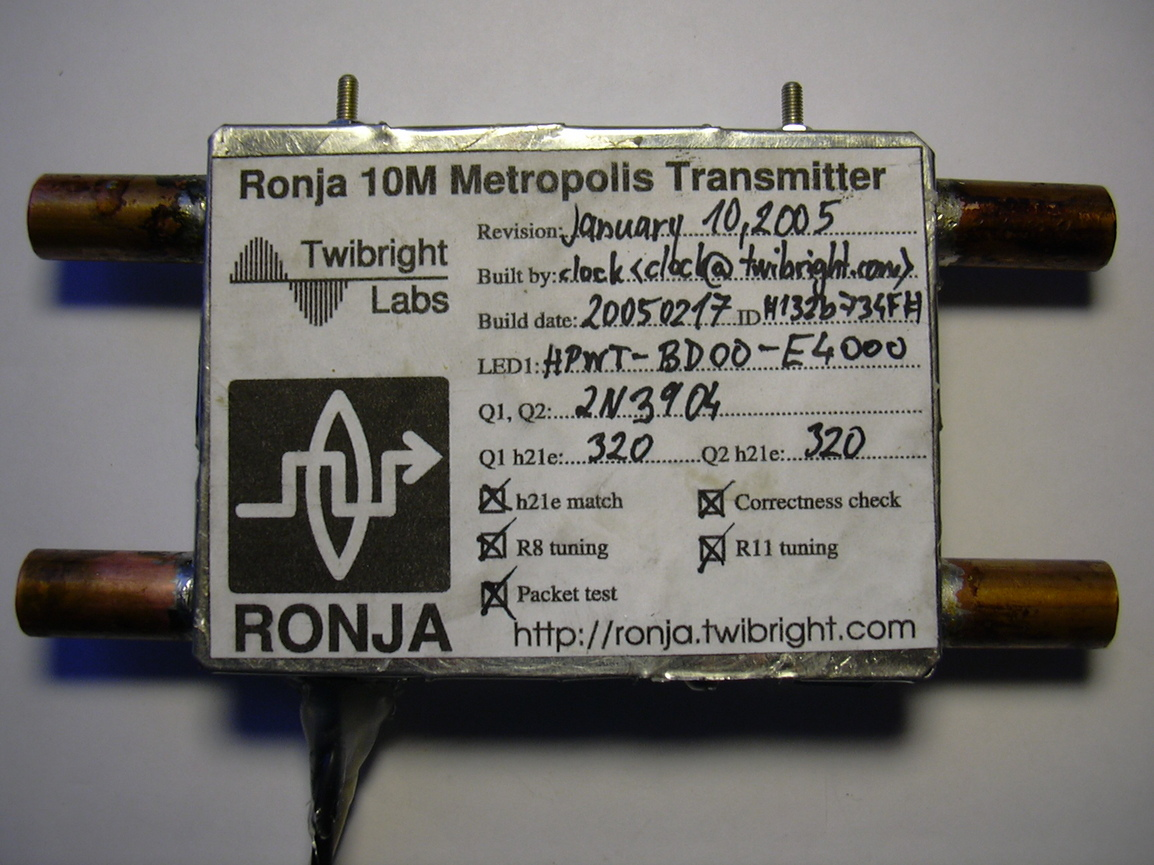
\includegraphics[scale=0.85]{transmisor/1b80}
    \caption{Transmisor Ronja 10M Metropolis}
  \end{figure}
\end{frame}

\begin{frame}{Hardware mecánico}
  \begin{figure}
    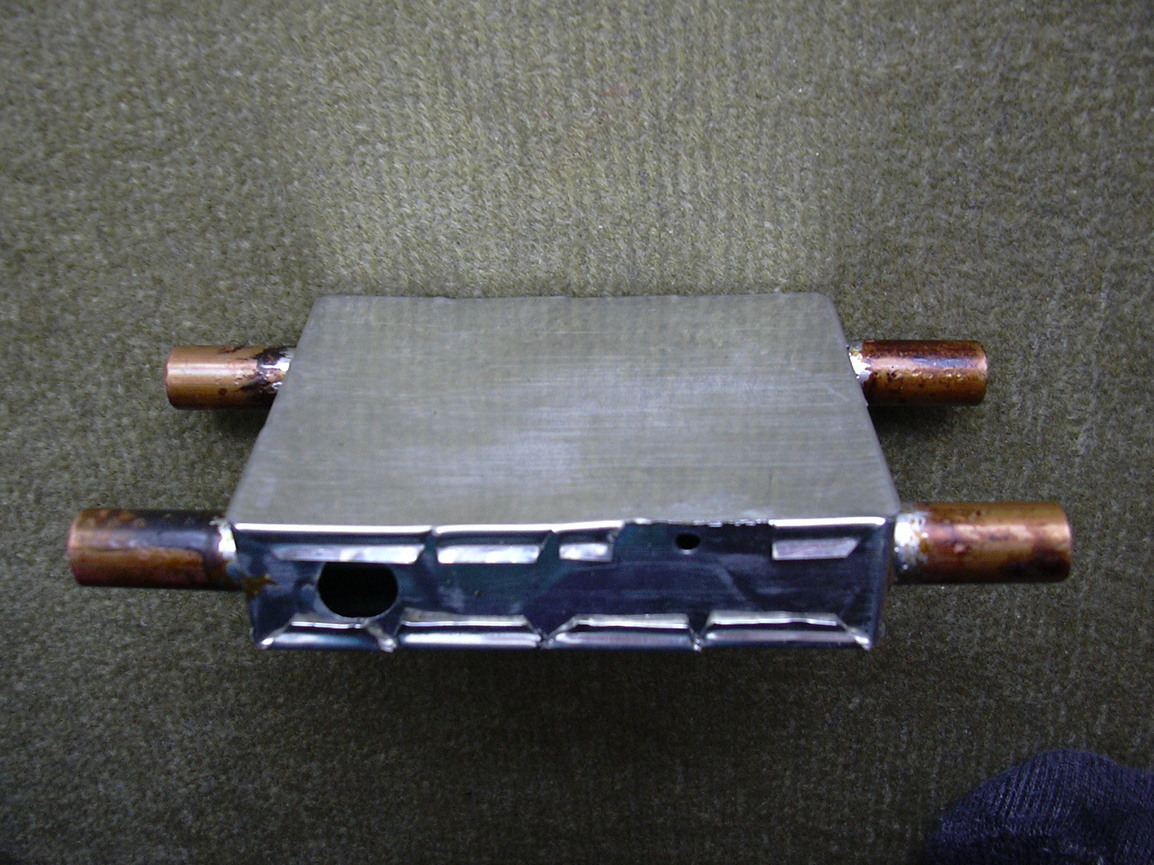
\includegraphics[scale=0.9]{transmisor/1b50}
  \end{figure}
\end{frame}

\begin{frame}{Diseño Hardware mecánico}{Hecho en \alert{qcad} - \url{http://www.ribbonsoft.com/qcad_downloads.html}}
  \begin{figure}
    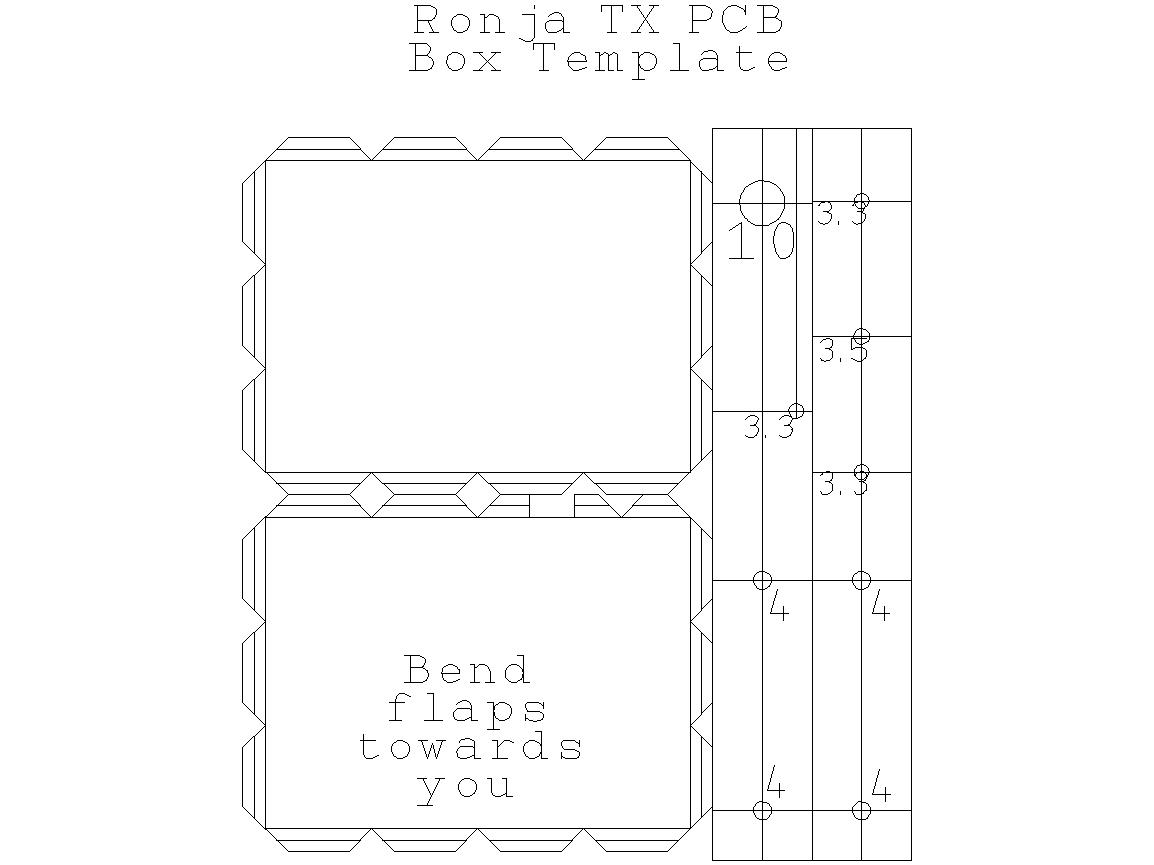
\includegraphics[scale=0.225]{transmisor/tx_pcb2}
  \end{figure}
\end{frame}

\begin{frame}{Hardware mecánico}
  \begin{figure}
    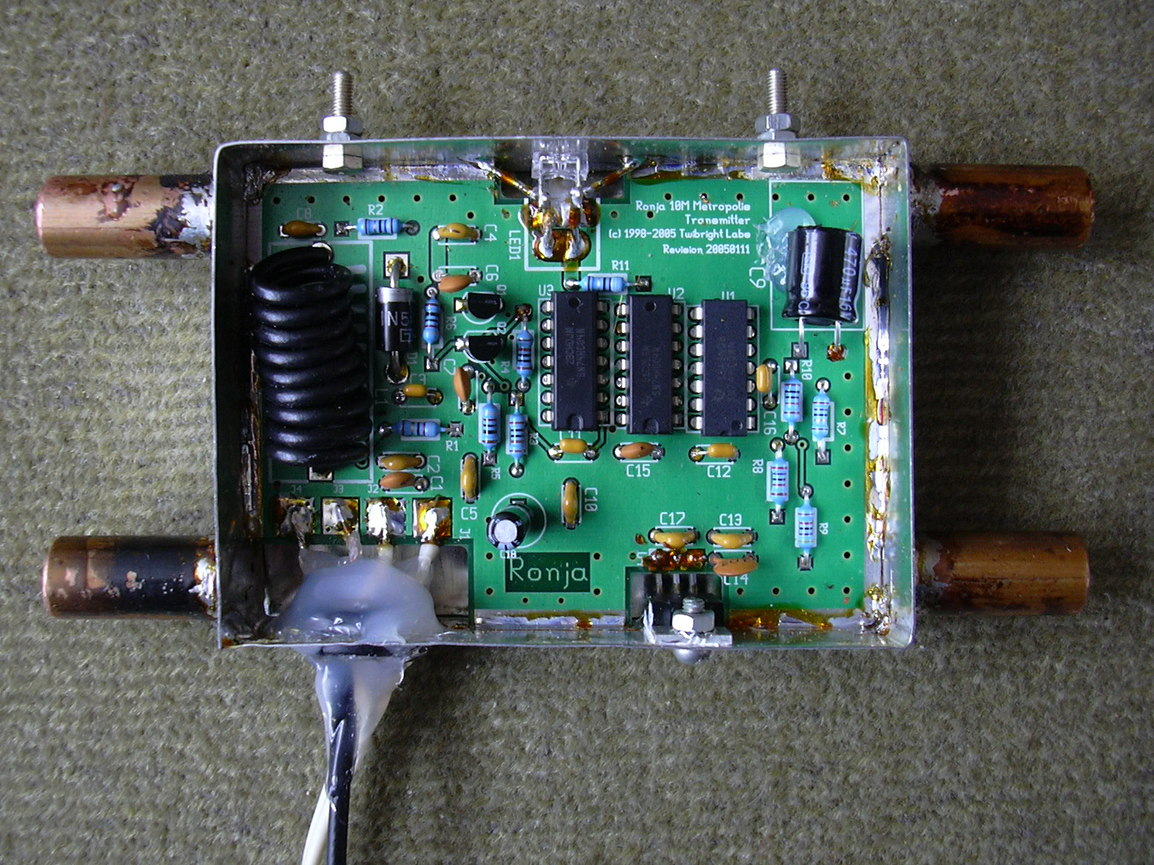
\includegraphics[scale=0.85]{transmisor/1b76}
    \caption{Dentro esta el Hardware electrónico}
  \end{figure}
\end{frame}

\begin{frame}{Hardware electrónico}
  \begin{figure}
    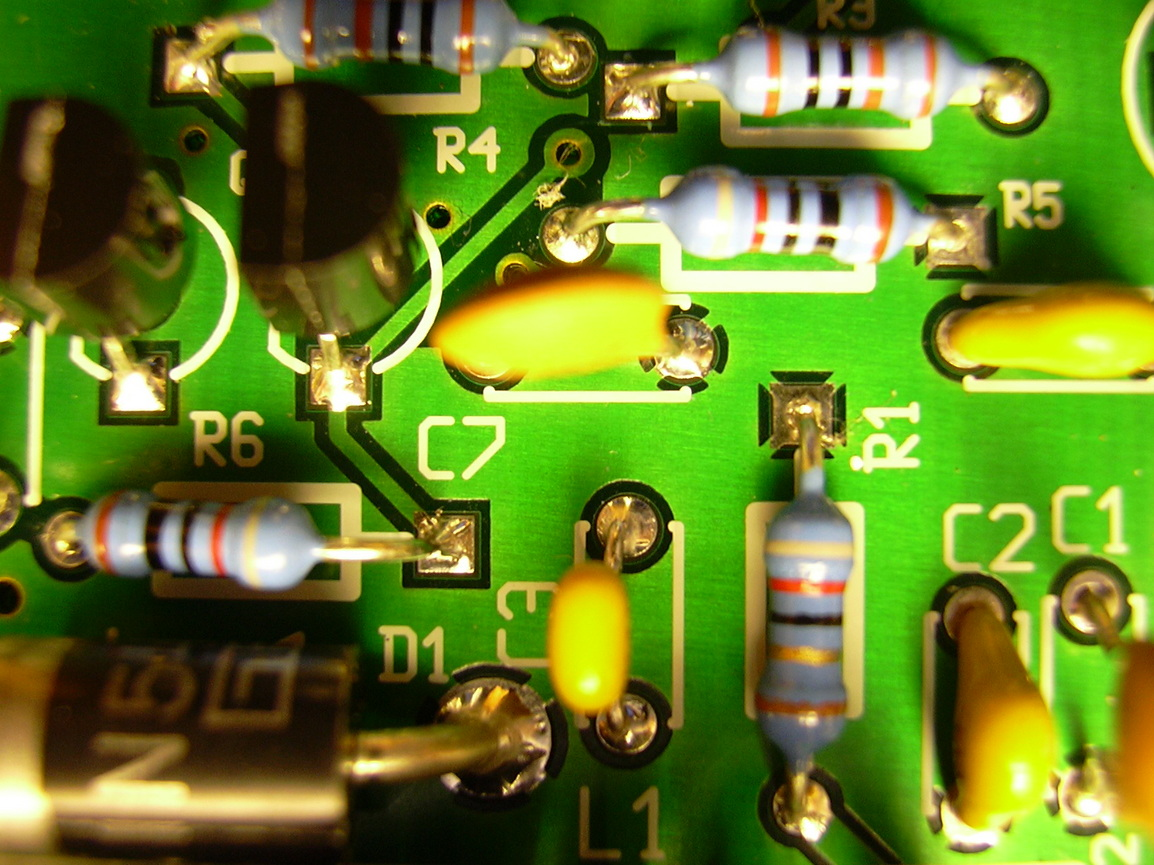
\includegraphics[scale=0.85]{transmisor/1b84}
    \caption{Tarjeta con dispositivos electrónicos}
  \end{figure}
\end{frame}

\begin{frame}{Hardware electrónico}
  \begin{figure}
    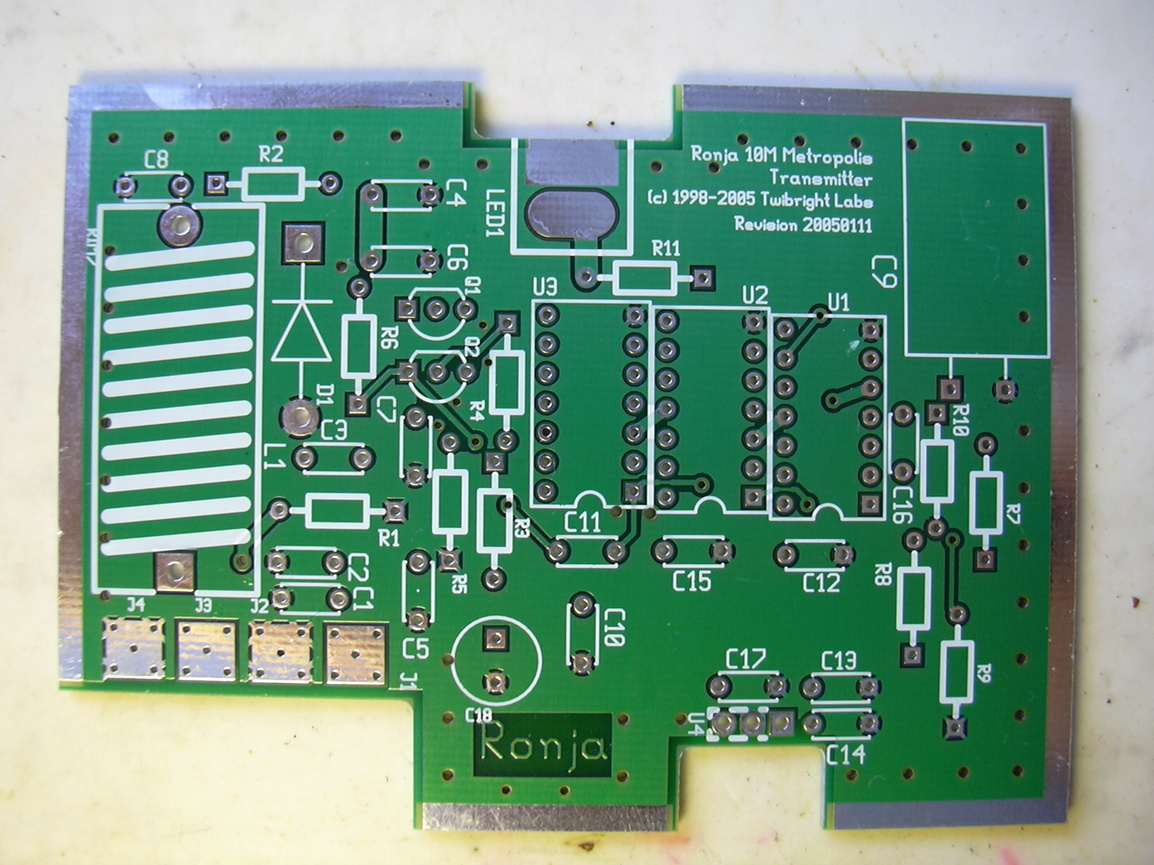
\includegraphics[scale=0.85]{transmisor/1b5e}
    \caption{Tarjeta de circuito impreso (PCB)}
  \end{figure}
\end{frame}

\begin{frame}{Hardware electrónico}{Se visualiza con \alert{gerbv} - \url{http://gerbv.sourceforge.net}}
  \begin{figure}
    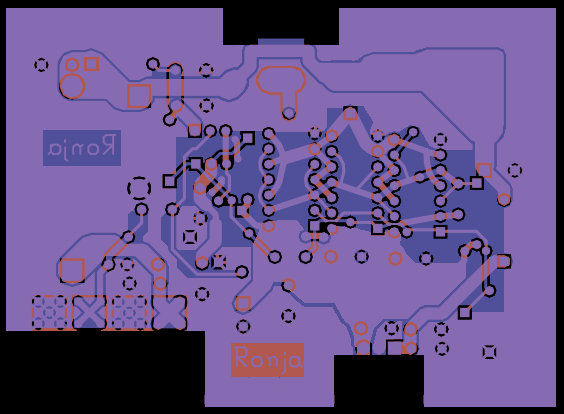
\includegraphics[scale=0.4]{transmisor/transmisor_gerber.png}
    \caption{Archivo gerber}
  \end{figure}
\end{frame}

\begin{frame}{Diseño de Hardware electrónico}{Se edita con \alert{pcb} - \url{http://pcb.gpleda.org}}
  \begin{figure}
    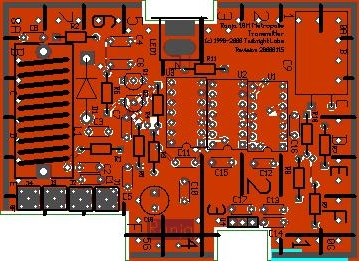
\includegraphics[scale=0.65]{transmisor/metropolis_transmitter}
    \caption{Archivo PCB}
  \end{figure}
\end{frame}

\begin{frame}{Diseño de Hardware electrónico}{Creado con \alert{gEDA/gschem} - \url{http://www.gpleda.org}}
  \begin{figure}
    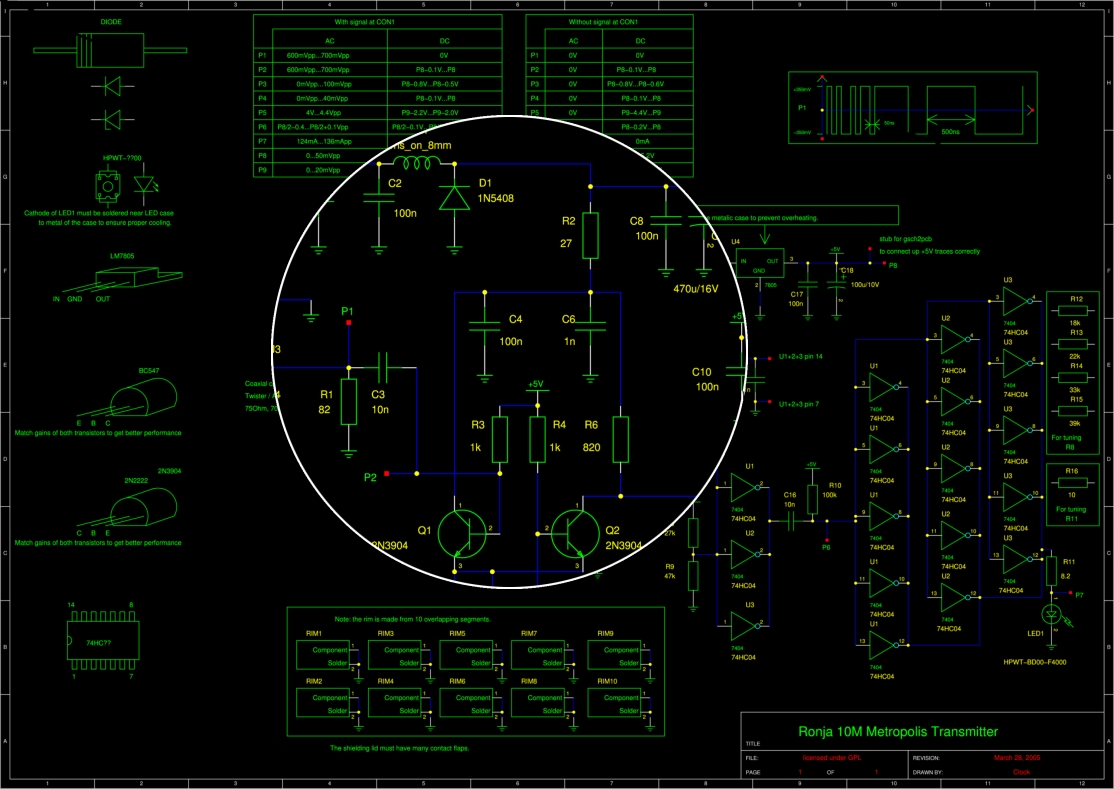
\includegraphics[scale=0.21]{transmisor/transmisor_esquema}
    \caption{Archivo del diagrama esquemático}
  \end{figure}
\end{frame}

\begin{frame}{Producción de Hardware}
  \begin{figure}
    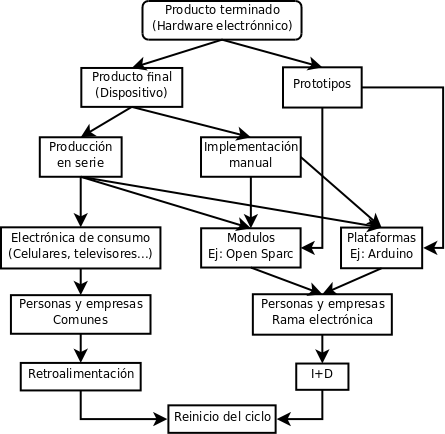
\includegraphics[scale=0.3]{img/objetivos}
    \label{fig:objetivos}
    \caption{Objetivos de los productos}
  \end{figure}
\end{frame}
 
\section{Que es Open Source Hardware}
%DISPONIBILIDAD DE LOS COMPONENTES
\subsection{Definiciones formales}

\begin{frame}{Free hardware design}{Libre hardware design}
  \begin{itemize}
  \item Se refiere a un diseño que se puede copiar, distribuir, modificar y fabricar libremente.
  \item Libre para hacer claridad que es libre y no gratis.
  \end{itemize}
\end{frame}

\begin{frame}{Open source hardware}
  \begin{itemize}
  \item Se refiere al hardware que tiene disponible toda su información de diseño.
  \item El Open Source Hardware puede estar basado en Free Hardware Design.
  \item o también en diseños que no son totalmente libres.
  \end{itemize}
\end{frame}

% \begin{frame}{No hay hardware libre}
%   Como hay una diferenciación entre el diseño y la implemntación no se debe usar el termino porque no es claro.
%   \item No se debe usar el termino Free Hardware.
% \end{frame}

\begin{frame}{Open Hardware}
  \begin{itemize}
  \item Es marca registrada del Programa Open Hardware Specification.
  \item Es una forma limitada de Open Source Hardware
    \begin{itemize}
    \item Garantiza la disponibilidad de especificaciones para escribir controladores para el dispositivo.
    \end{itemize}
  \end{itemize}
\end{frame}

\begin{frame}
  \begin{figure}
    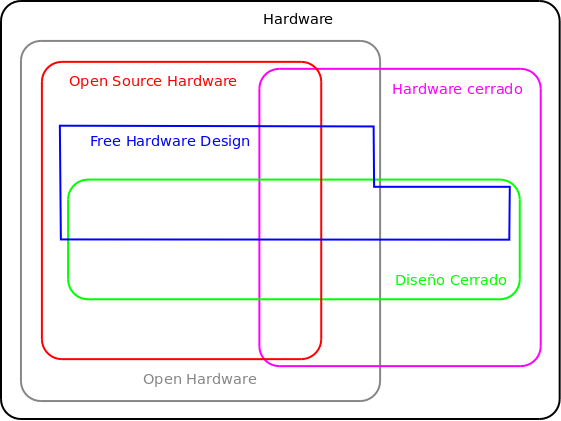
\includegraphics[scale=0.3]{img/categorias}
    \caption{Categorías de hardware}
    \label{fig:categorias}
  \end{figure}
\end{frame}

\begin{frame}{Problemas y restricciones}{Herramientas y formatos ECAD}
  \begin{itemize}
  \item Históricamente los formatos han estado ligados al software.
  \item EDIF estandar fallido.
  \item No hay un formato estandar aceptado para intercambio de archivos ECAD.
  \item Práctica común de compartir imágenes.
    \begin{itemize}
    \item Aunque no son editables con las herramientas que fueron creadas son consideradas código fuente.
    \end{itemize}
  \end{itemize}
\end{frame}

\begin{frame}{Problemas y restricciones}{Herramientas y formatos ECAD}
  \begin{table}
    \begin{tabular}{|c|c|c|}
      \hline
      Software & \multicolumn{2}{c|}{Formato Nativo\footnote{Si es imágen se debe reescribir}}\\
       & Abierto\footnote{Libre o estandar} & Cerrado\\
      \hline
      Libre & 0 & 1\\
      Gratis & 2 & 3\\
      Pago & 4 & 5\\
      \hline
    \end{tabular}
    \caption{Niveles de restricción}
    \label{tab:niveles}
  \end{table}
\end{frame}

\subsection{Para que el Open Source Hardware}

\begin{frame}{Globalización y sociedad del conocimiento}
  \begin{figure}
    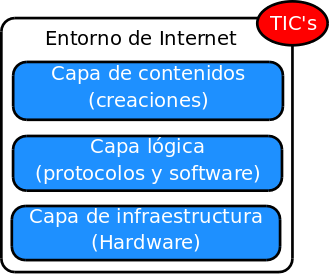
\includegraphics[scale=0.3]{img/internet}
    \label{fig:internet}
    \caption{Modelo de descripción y descomposición de Internet en capas \cite{Bercelli}.}
  \end{figure}
\end{frame}

\begin{frame}{Modelo del Software Libre}
  \begin{itemize}
  \item Garantiza a cualquier persona derechos para usar, estudiar, modificar y compartir el software.
  \item La garantía se establece legalmente con un contrato (Licencia).
%  \item Permite la democratización de los medios de producción.
  \item Procura el uso de protocolos estandar.
  \item Abre la capa lógica a la sociedad del conocimiento.
  \end{itemize}
  \begin{figure}
    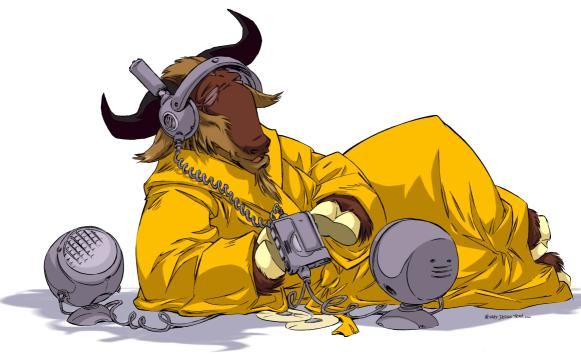
\includegraphics{img/listen-eighth}
  \end{figure}
\end{frame}

\begin{frame}{Cultura Libre}
  \begin{itemize}
  \item Extensión del modelo del software libre.
  \item Garantiza el derecho a compartir los recursos culturales.
  \item También se hace por medio de licenciamiento.% \cite{cc}.
  \item Abre la capa de contenidos a la sociedad del conocimiento.
  \end{itemize}
\end{frame}

% Carolina Botero.

% Diff, sl codigo libertad modificar código
% cl importancia fomentar una cultura de compartir entre las personas los recursos culturales frente a una cultura de control de copia que es la que favorece un sistema de derecho de autor tradicional.
% diff en cl no necesariamente se debe permitir la modificación, ya con compartir es cultura libre.


% garantiza la posibilidad de circuolar los objetos culturales
% definicones de cultura que tienen que ver con


%Gabriel Zea

% %3476741
% Ejercer el derecho que tiene para ver las obras

% libertad de acceso al conocimiento y producción cultural, patrimonio de la gente en últimas, el acceso a la cultura no debia estar regulado por trabas financieras, debería poder acceder al contenido cultural como aacceder a un servicio básico.

% Uno debería poder acceder ala cultura sin ningún tipo de barrera, del que lo ve.
% Del productor cultural, en donde se produce la cultura en medios económicos hay mucha presion donde hay mucha presión y en últimas no es libre de crear entonces esta es satisfaciendo el mercado bajo presión, sin esa presión realmente crearía.

% yokoman, no es música de baile, raya lo experimental que usa discursos chavistas para hacer las piezas, no podría circular sus piezas en un entorno comercial. entonces lo que hace es ejercer su libertadf de creador y darle la oportunidad a otras personas de hacer lo mismo.

% Los ceradores culturales y los artistas buscan la felicidad a partir de la creación, así ser feliz no valla de la mano de lo económico, clave de la cultura libre para crear.

% Wired sobre arduino
% pillar el blog de arduino, artículo como de hace 3 meses. wiring en colombia, coincidencialmente tien que ver con el arte y el diseño, que lo enmarca en el terreno de la creación libre. proccesing, en los 90 principios de 2000 el arte elctrónico se hizo con privativo, los etos en la creación digital son muy marcados. el asunto se volvio asficciante, entonces proccesing se lanza independiente sin ningun compormiso software  libre y entnoces boom de gente que usa el proyecto y contribuye. El bom se da en el arte y luego toca el terreno de la ingeniería. Entonces nace wiring como sistema de prototipado compatible como procesing, aplano el terreno para que apareciera arduino, las librerias base para wiring y cean una plataforma de hardware acesible que cualquier persona pudiera crear y usarla Arduino, de nuevo boom en el campo artístico. se convierte casí en un estandar en el campo del diseño, arte y música, genera un eto pero como es abierto el eto también esta abierto.

\begin{frame}{Open Source Hardware}
  \begin{itemize}
  \item Para abrir la capa de infraestructura se deben tener en cuanta:
    \begin{itemize}
    \item Free Hardware Design.
    \item Open Source Hardware
    \end{itemize}
  \item El modelo del software libre se puede extender hasta Free Hardware Design.
  \item Debe usarse otro modelo para la implementación de Open Source Hardware.
    % Modelo de negocio como en software Libre, basado en servicios y no en el constructo físico.
  \end{itemize}
\end{frame}

\section{Proyectos de Open Source Hardware}

\subsection<presentation>*{Nivel de restricción}


\begin{frame}{Openmoko}{\url{http://www.openmoko.com}}
  \begin{figure}
    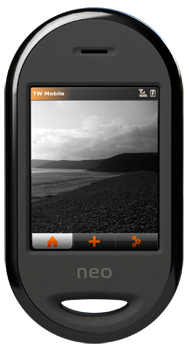
\includegraphics[scale=0.65]{img/freerunner_shop1}
    \caption{Teléfono móvil.}
    \label{fig:openmoko}
  \end{figure}
\end{frame}

\begin{frame}{The Open Graphics Project}{\url{http://opengraphics.org}}
  \begin{figure}
    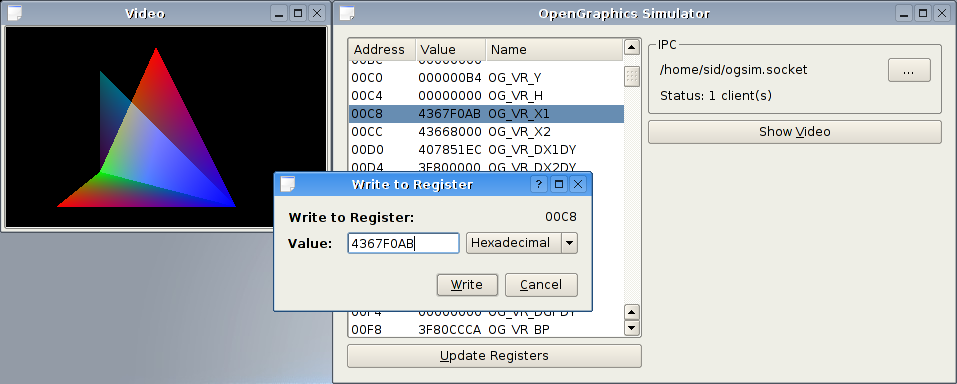
\includegraphics[scale=0.35]{img/ogsim-screen1}
    \caption{Tarjeta de video.}
    \label{fig:ogp}
  \end{figure}
\end{frame}

\begin{frame}{Open sparc}{\url{http://www.opensparc.net}}
  \begin{figure}
    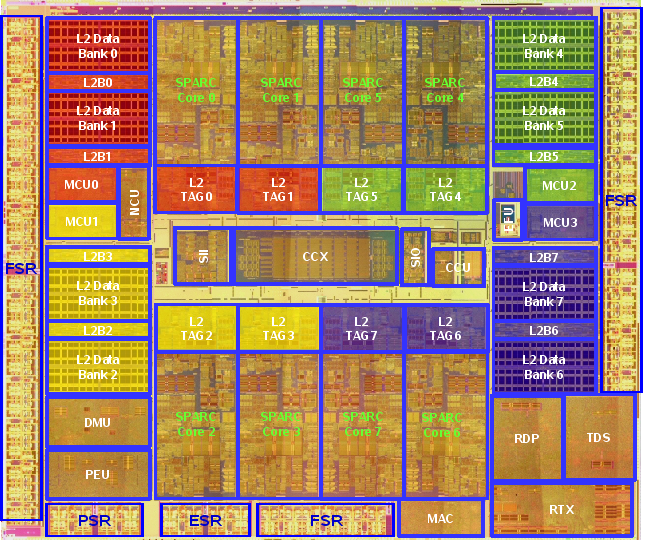
\includegraphics[scale=0.4]{img/ultrasparc-t2-layout}
    \caption{Procesador de 64 bits.}
    \label{fig:opensparc}
  \end{figure}
\end{frame}

\begin{frame}{Ronja}{\url{http://ronja.twibright.com}}
  \begin{figure}
    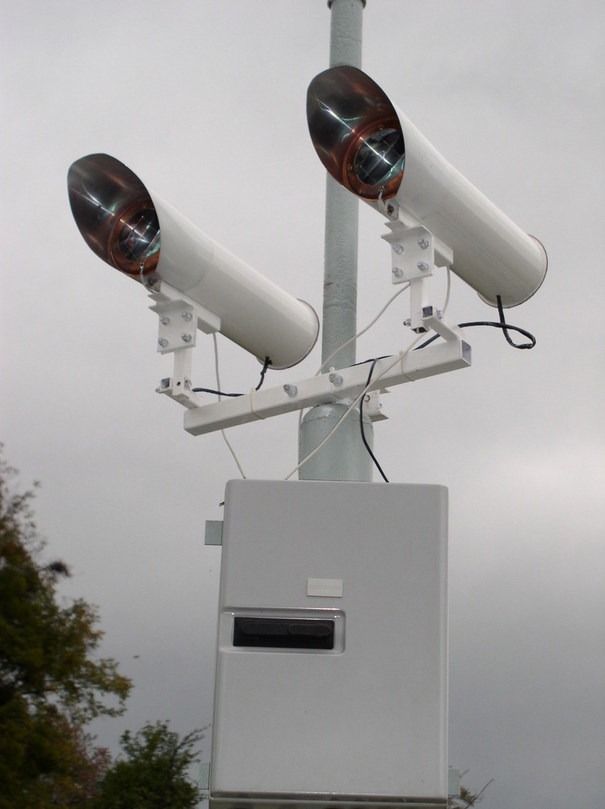
\includegraphics[scale=0.22]{img/122e}
%    \caption{Nivel de restricción 0}
    \label{fig:ronja}
  \end{figure}
\end{frame}

\begin{frame}{RobotCub}{\url{http://www.robotcub.org}}
  \begin{figure}
    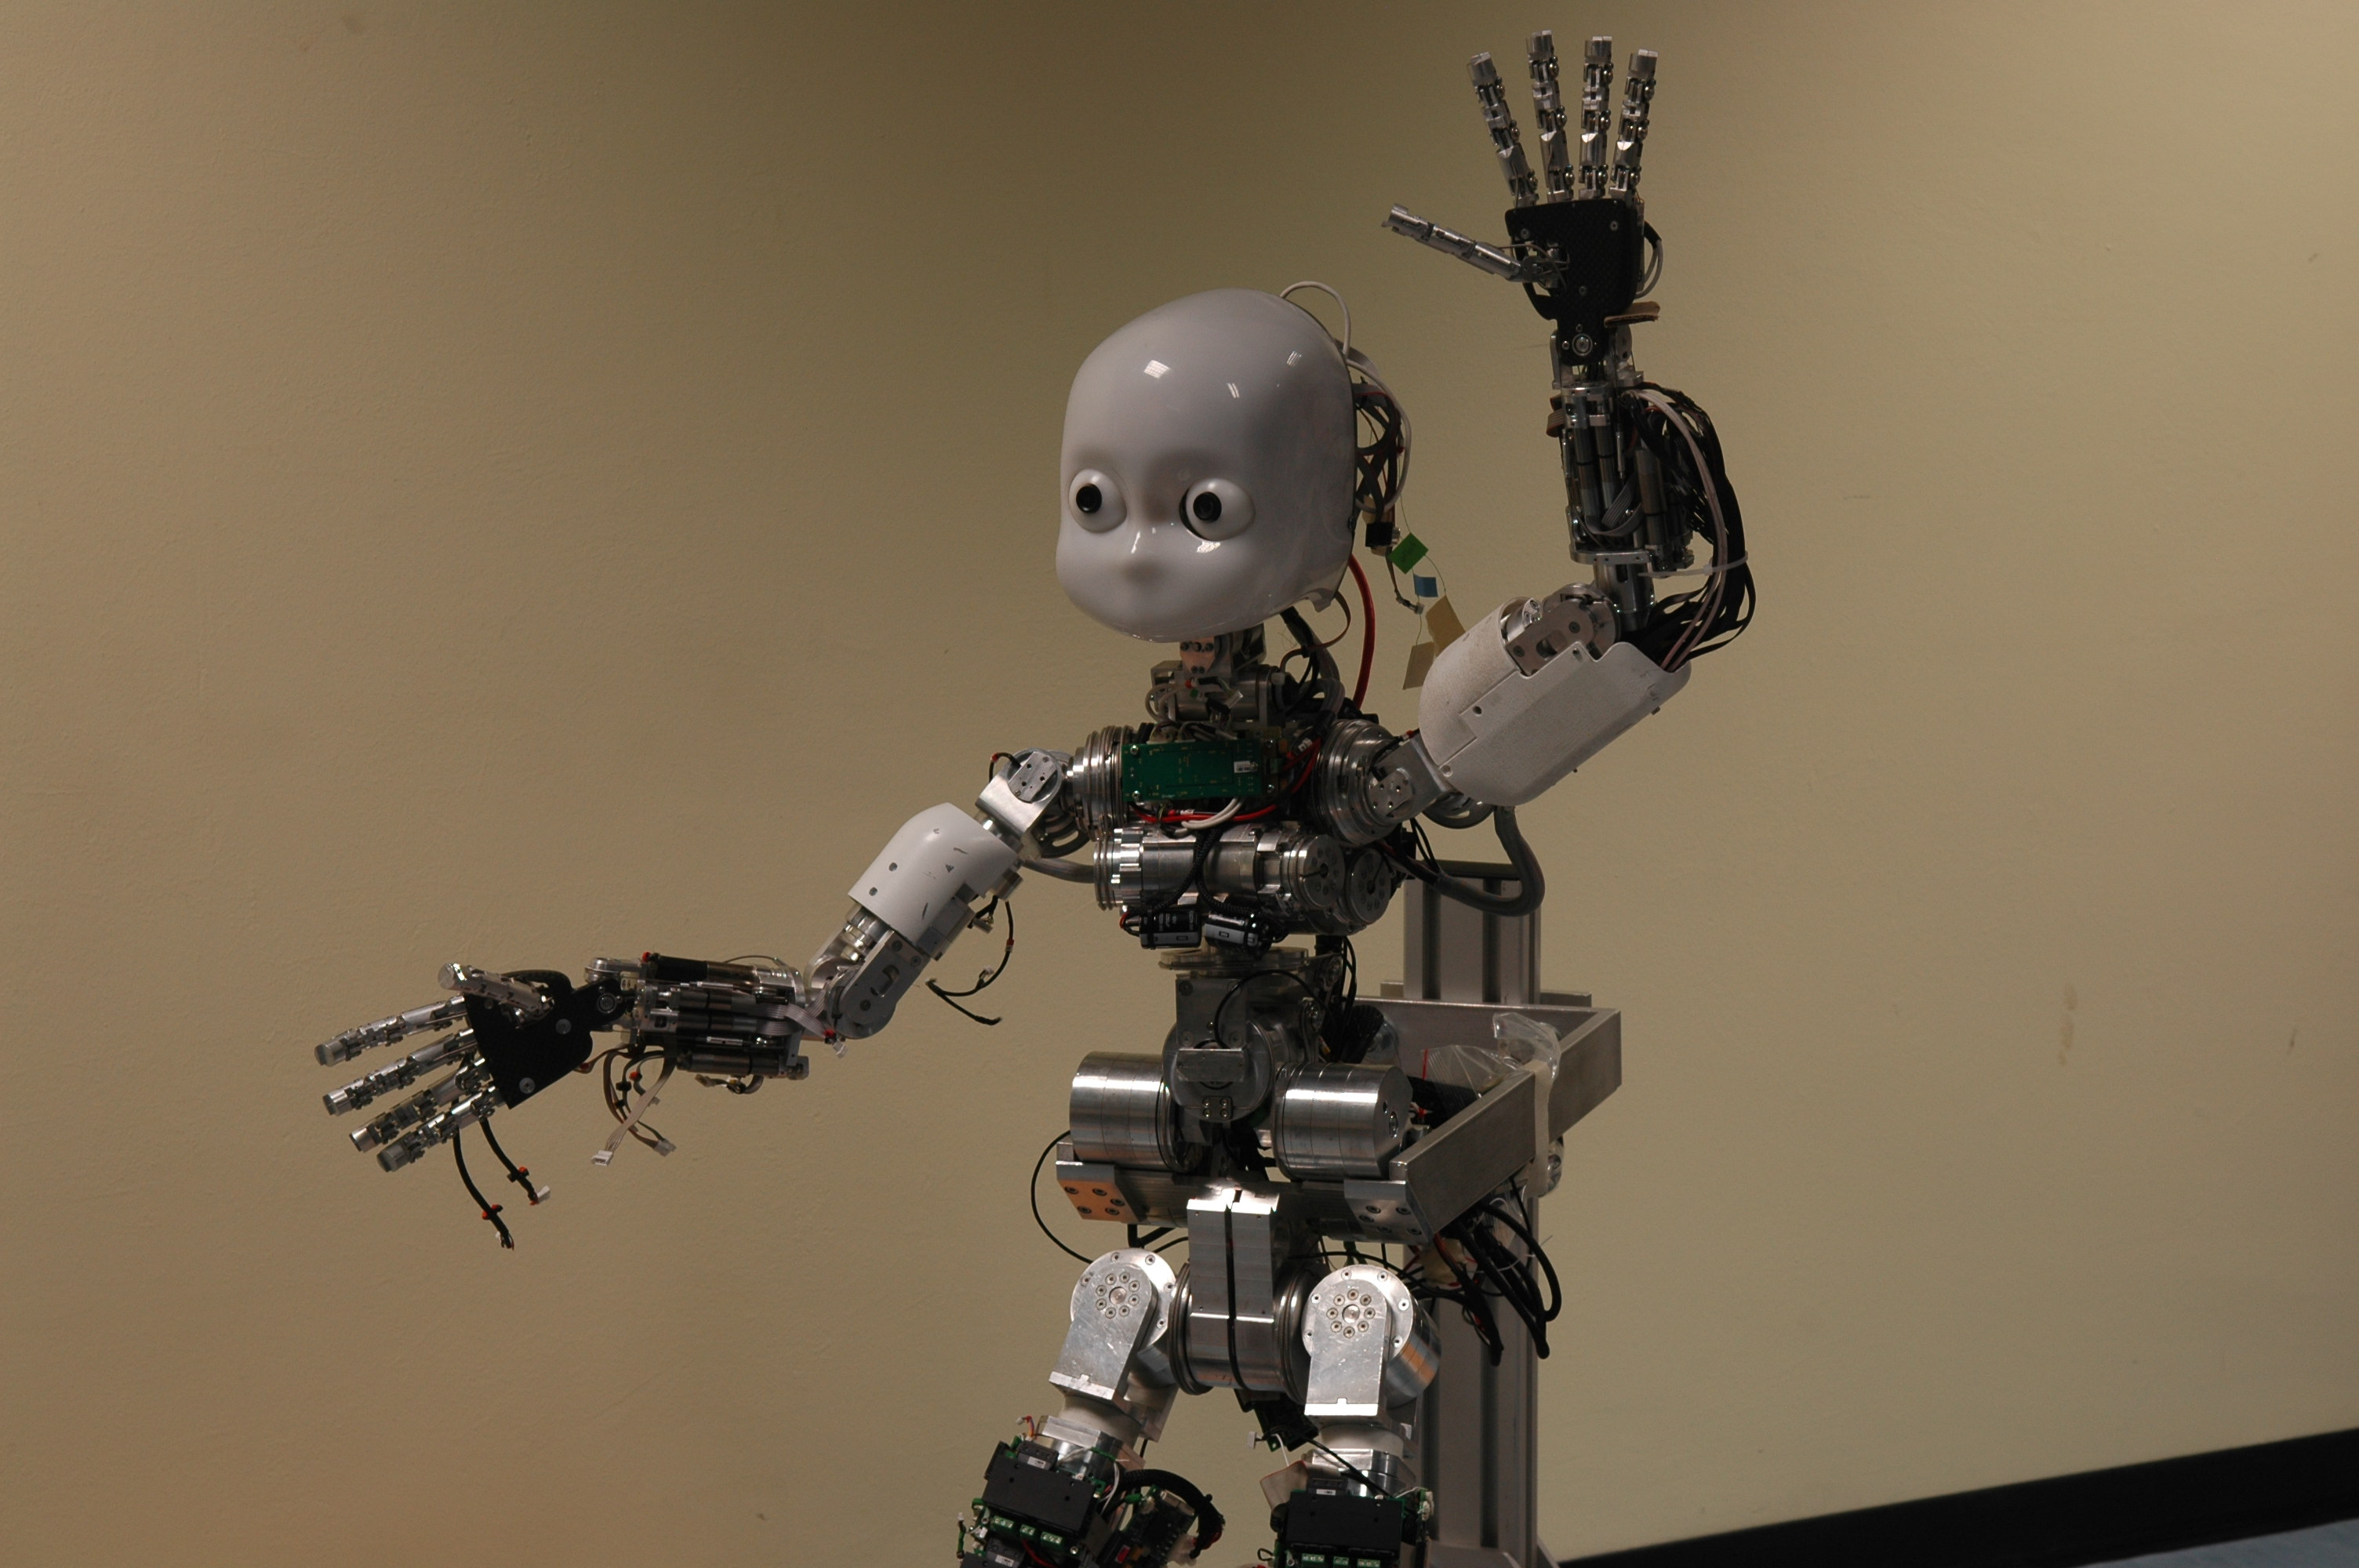
\includegraphics[scale=0.085]{img/DSC_3997}
    \caption{iCub.}
    \label{fig:icub}
  \end{figure}
\end{frame}

\begin{frame}{ECB AT91 V2}{\url{http://www.emqbit.com}}
  \begin{figure}
    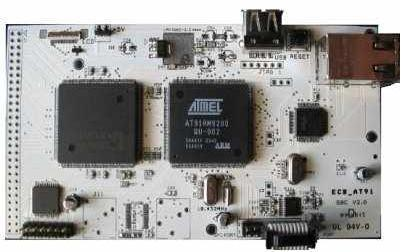
\includegraphics[scale=0.6]{img/V2}
    \caption{Free open SBC design Single Board.}
    \label{fig:ecb}
  \end{figure}
\end{frame}

\begin{frame}{Arduino}{\url{http://www.arduino.cc}}
  \begin{figure}
    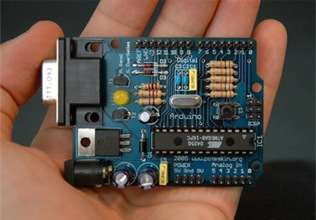
\includegraphics[scale=0.6]{img/arduino316}
    \caption{Plataforma para prototipado.}
    \label{fig:arduino}
  \end{figure}
\end{frame}

% \begin{frame}{slide}
%   % Diferencias HW L y HW C
% %   \begin{itemize}
% %   \item Modelo cerrado...
% %   \item Modelo abierto... el desarrollo con modelo abierto va hacía... será parte de tu vida y no lo sabías
% %   \end{itemize}
%   Nombrar proyectos\\
%   Cuadro (Matriz de los proyectos y que tipo de hardware ``libre'' es..)
% \end{frame} 

\section<presentation>*{Extendiendo el modelo del software libre al hardware}

\begin{frame}{Conclusiones}
  \begin{block}{}
    \begin{itemize}
    \item El Diseño de hardware es un proceso que esta al alcance de todos, tiene grandes alcances y es importante buscar modelos que lleven el diseño a la producción en masa.
    \item Ya existen varios proyectos de gran envergadura que son Open Source Hardware.
    \item Hay un grave problema de interoperabilidad entre formatos y herramientas.
    \end{itemize}
  \end{block}
\end{frame}

\begin{frame}{Agradecimientos}
  \begin{itemize}
  \item Karel ``Clock'' Kulhavý - Ronja.
  \item Graham Seaman - Open Collector.
  \item Andres Calderon - emQbit.
  \item Carolina Botero.
  \item Gabriel Zea.
  \item Coordinadores de Campus Party/Software Libre.
  \end{itemize}
\end{frame}

\appendix

\section<presentation>*{\appendixname}

\begin{frame}
  \frametitle<presentation>{Bibliografía I}
  \begin{thebibliography}{99}
    \beamertemplatebookbibitems
  \bibitem[1]{PardoBoluda}Fernando Pardo Carpio y José A. Boluda Grau
    \newblock \emph{VHDL, Lenguaje para síntesis y modelado de circuitos, 2a. edición}
    \newblock Alfaomega, 2004
  \bibitem<1->[Bercelli 2006]{Bercelli}Ariel Bercelli
    \newblock \emph{Aprender la Libertad}
    \newblock 2006
    \newblock \url{http://www.aprenderlalibertad.org/libro-all}
  \end{thebibliography}
\end{frame}

\begin{frame}
  \frametitle<presentation>{Bibliografía II}
  \begin{thebibliography}{99}
    \beamertemplatearticlebibitems
  \bibitem<1->[Güichal 2005]{Guillermo}Guillermo Güichal
    \newblock \emph{Diseño Digital Utilizando Lógicas Programables}
    \newblock Junio 29, 2005
    \newblock \url{http://fpga.com.ar/notas/NotasCompletas.pdf}
  \bibitem<1->[4]{clasificacion}Ivan González, Juan González y Francisco Gómez-Arribas
    \newblock \emph{Hardware libre: clasificación y desarrollo de hardware reconfigurable en entornos GNU/Linux}
    \newblock 6 de Septiembre de 2003
    \newblock \url{http://www.iearobotics.com/personal/juan/publicaciones/art4/hardware-libre.pdf}
  \end{thebibliography}
\end{frame}

\begin{frame}[allowframebreaks]
  \frametitle<presentation>{Infografía}
  \begin{thebibliography}{99}
    \beamertemplatearticlebibitems
  \bibitem[5]{Ales}\emph{gEDA - GPL Electronic Design Automation}, \url{http://www.geda.seul.org/talks/deluge_ales.pdf}
  \bibitem<1->[6]{ronja}\emph{Ronja 10M Metropolis Transmitter}, \url{http://ronja.twibright.com/transmitter/index.php}
  \bibitem<1->[7]{definiciones}\emph{Definitions}, \url{http://www.opencollector.org/Whyfree/definitions.html}
  \bibitem<1->[8]{openhardware}The Open Hardware Certification Program, \url{http://web.archive.org/web/20010203155900/www.openhardware.org/}
  \bibitem<1->[9]{freesoftware}\emph{La definición de Software Libre}, \url{http://www.gnu.org/philosophy/free-sw.es.html}
    % \item Charlas de Fredy y Jorge
  \end{thebibliography}
\end{frame}

\section<presentation>*{Sobre este documento}

\begin{frame}
  \begin{block}{Licencia}
    \begin{figure}
      
\includegraphics[scale=0.9]{img/by-sa}
    \end{figure}
    \centering
    \small Creative Commons Atribución-Compartir Obras Derivadas Igual 2.5 Colombia
    \small \url{http://creativecommons.org/licenses/by-sa/2.5/co}
\end{block}
\begin{block}{}
  Creado con \LaTeX/Beamer
\end{block}
\end{frame}

\end{document}
